\documentclass[a4paper,11pt]{article}

%\usepackage[utf8]{inputenc}
\usepackage[frenchb,english]{babel}
%\usepackage[T1]{fontenc}
%\usepackage{lmodern}
\usepackage{hyperref}
\hypersetup{colorlinks=false}
\usepackage{graphicx}
\usepackage{subfigure}
\usepackage{longtable,geometry}
%\pagestyle{headings}
%\geometry{dvips,a4paper,margin=2cm}
\selectlanguage{english}

\geometry{verbose,a4paper,tmargin=30mm,bmargin=20mm,lmargin=15mm,rmargin=15mm}


\begin{document}

\title{Using the OpenFEC.org Performance Evaluation Tools}

\author{Vincent Roca (INRIA), Jonathan Detchart (INRIA), Mathieu Cunche (INRIA)\\
	Valentin Savin (CEA-LETI), J\'er\^ome Lacan (ISAE)\\
	\emph{http://openfec.org}}
\date{\today} 

\maketitle
\tableofcontents

\vfill

\noindent version: \date{\verb;$Id: howto_performance_evaluation.tex 109 2014-04-08 09:10:12Z roca $;
\newpage


\section{Introduction}
%---------------------

%\subsection{What are the performance evaluation tools ?}
%-------------------------------------------------------

The performance evaluation tools are a set a Perl scripts meant to assess the code and codec
performances, using many different metrics, in an automatic way.


\subsection{Principles}
%----------------------

These scripts use the \verb+eperftool+ program to simulate a transmission between a sender
and a receiver over a lossy channel. Therefore, we are doing an actual AL-FEC encoding (using
a real encoder), and an actual AL-FEC decoding (using a real decoder). Only the transmissions
are simulated.
You, as the user, control many parameters, like the transmission type (in which order should
the source and repair packets for the various blocks be transmitted), the loss probability,
and all the code specific parameters (e.g. the object size, code-rate, symbol size).

A first script, \verb+run_tests.pl+, runs several iterations of the \verb+eperftool+ program
with the desired parameters.
All test results are written into log files. These log files are then analyzed in real-time and
the results are inserted into a database that can be either a {\bf MySQL database} or an
{\bf SQLite file}.

A second script, \verb+generate_graph.pl+, is used to create the curves using various kinds of
metrics (e.g. you can have several kinds of curves without having to re-run tests).
This script connects to the database to execute \verb+select+ SQL requests and generates
\verb+gnuplot+ files (\verb+.dem+ for the \verb+gnuplot+ commands and \verb+.dat+ for the raw data).
In no case does the script modify the database itself, so you even run it during tests, to
generate preliminary curves.

Both scripts need a parameter file (e.g. \verb+params.txt+, but you can rename it as you want).
This ASCII file contains all the necessary parameters to run tests and to generate the curves
(even if in the latest case, only the database connection string is required).


\subsection{Requirements and limits}
%-----------------------------------

\begin{itemize}
\item
The set of tools provided require you use a {\bf Linux or Mac OSX operating systems}.
This does not mean it won't work on different operating systems, just that we did not
test and cannot guaranty anything.
\item
Performance analysis tools require you use either a MySQL or SQLite tools. Make
sure one of them is available on your system, otherwise install it.
See section~\ref{sec:sql_config} for more information.
\item
LDPC matrices plot facilities have specific requirements. 
See section~\ref{sec:plot_matrices} for more information.
\end{itemize}

%\newpage


%-------------------------------------------------------------------------------

\section{Configuring the "params.txt" file}
%----------------------------------------
\label{sec:params_file}
\begin{flushright}
\framebox{
\begin{minipage}{10cm}
	\emph{$\rightarrow$ In short:
	edit the "params.txt" file to define the simulation parameters.
	}
\end{minipage}
}
\end{flushright}

The parameters file (called by default \verb+params.txt+) contains the following sections:
\begin{itemize}
\item \emph{Tools:} paths to the various tools;
\item \emph{Files:} paths to the various files that may be needed during simulations;
\item \emph{Tests:} tests to perform;
\item \emph{Code/codec configuration:} codes to use and how to use them;
\item \emph{Transmission and loss configuration:} kind of channel to use;
\item \emph{Database configuration:} SQL related parameters; 
\end{itemize}

\noindent See the provided file for explanations on the syntax. The present document only
contains additional information not present in the \verb+params.txt+ file.


% \subsection{The "Tools" section}
% %-------------------------------
% 
% The Tool part defines the paths to all the executable tools that are (or may be) used by the first script.
% \begin{table}[ht]
% \begin{center}
% \begin{tabular}{|r|l|}
% \hline
% Name & Description\\
% \hline \hline
% fec\_tool &  Path to the \verb+eperftool+ executable\\
% qc2mod2sparse & QC-LDPC only: path to the QC tool that expends a base circulant matrix into H\\
% \hline
% \end{tabular}
% \end{center}
% \end{table}
% 
% The \textbf{fec\_tool} parameter must contain a (relative or absolute) path for the \verb+eperftool+
% executable.
% You must use \verb+eperftool+ because the \verb+openfec_test.pl+ script parses the standard output to get some metrics like decoding starting/finishing times, the symbol size, the number of source symbols.
% 
% The \textbf{qc2mod2sparse} parameter is only meaningful with QC-LDPC codes.
% It must contain a (relative or absolute) path to the \verb+qc2mod2sparse+ executable.
% This tool is usued by the test script to convert a QC base circulant identity matrix file to a binary
% (A.K.A. "modulo 2") sparse matrix file, for a given expension factor.
% 
% 
% \subsection{The "Files" section}
% %-------------------------------
% 
% The "Files" part defines all files which are used by the first script.\\
% \begin{table}[ht]
% \begin{center}
% \begin{tabular}{|r|l|}
% \hline
% Name & Description\\
% \hline \hline
% matrix\_files & Set of matrix files used by QC codec\\
% trace\_file & Name of the trace file which contains all run tests with their results.\\
% \hline
% \end{tabular}
% \end{center}
% \end{table}
% 
% The \textbf{matrix\_files} parameter is optional. It must be a set of path to the differents matrix files separated by spaces. \\\textbf{Only if you are using the QC-LDPC with a specified matrix file codec.}\\
% \textbf{trace\_file} must be the name of a file (no special characters). At the end of tests, it constains all \verb+eperftool+ executions and their results.
% 
% 
% \subsection{The "Tests" section}
% %-------------------------------
% 
% The "Tests" part defines how tests are run, and how many tests are necessary for inserting data in database.\\
% \begin{table}[ht]
% \begin{center}
% \begin{tabular}{|r|l|}
% \hline
% Name & Description\\
% \hline \hline
% iteration & number of iterations for each test\\
% nb\_tests\_for\_partial\_results & number of tests before inserting the results into the database\\
% using\_threads & Allows script to run several tests at the same time by using threads\\
% using\_ml & Allows script to find the maximum loss for a given code. \\ & So, decoding will be a ML decoding.\\
% \hline
% \end{tabular}
% \end{center}
% \end{table}
% 
% The \textbf{iteration} parameter must be a positive integer.
% Each test is then done "iteration" times.
% 
% The \textbf{nb\_tests\_for\_partial\_results} must be a positive integer.
% For a given execution thread, every "nb\_tests\_for\_partial\_results" tests, the results are
% copied into a backup log file, processed, and the results inserted into the database.
% At the end of the thread, the whole backup log file is copied into the final log file.
% This approach is particularly useful in case of very long tests (e.g. that last
% several hours/days), in order to save partial results and get quickly an
% idea of the results (and possibly to change parameters if a mistake is found).
% 
% The \textbf{using\_threads} parameter must be a boolean (true or false).
% Set this parameter to true if you want to create multiple threads for running tests in
% parallel.
% By default, the script creates one thread per CPU core. For almost all tests, this is highly
% recommended since it makes simulations much faster.
% There's an exception though, when doing encoding/decoding speed tests. Here a single test must
% be run at a time for maximum accuracy. To do that, set this parameter to false.
% 
% The \textbf{using\_ml} parameter must be a boolean (true or false).
% This parameter is only used by LDPC and 1D-2D codecs.
% Set this parameter to true if you want to launch tests in such a way to trigger Maximum-Likelyhood
% (ML) decoding. This is useful to find the maximum erasure correction capabilities for a given
% LDPC code.
% To that purpose, the script computes the maximum number of recoverable losses for a given test, and
% executes \verb+eperftool+ accordingly. In this case, you dont need to define any loss with the "loss"
% parameter in the "transmission and loss configuration" section.
% 
% 
% \subsection{The "Code/codec configuration" section}
% %--------------------------------------------------
% 
% The "Code configuration" part defines all code and codec parameters.\\
% \begin{table}[ht]
% \begin{center}
% \begin{tabular}{|r|p{10cm}|c|}
% \hline
% Name & Description & Format\\
% \hline \hline
% \hline \multicolumn{2}{|c|}{\emph{General}} \\ \hline
% codec			& codec to use (e.g. RS, LDPC\_staircase, QC-LDPC) & list\\
% symbol\_size		& size of (source and repair) symbols, in bytes & list\\
% nb\_source\_symbols	& list of the number of source symbols to consider & min ~ max ~ step\\
% code\_rate		& code rate to use (mutually exclusive with nb\_repair\_symbols) & list\\
% nb\_repair\_symbols	& list of the number of repair symbols to consider (mutually exclusive with
% 			code\_rate) & list\\
% \hline \multicolumn{2}{|c|}{\emph{Code/codec specific}} \\ \hline
% ldpc\_N1		& Number of entry "1" for each row in the parity matrix\\ & (only for LDPC codecs)\\
% matrix\_mode		& Specify the type of matrix for QC codec (only for QC codec)\\
% qc\_matrix\_files	& Matrix files to use for tests\\
% exp\_factor		& Set of expension factor for QC matrix\\
% \hline
% \end{tabular}
% \end{center}
% \end{table}
% 
% The \textbf{symbol\_size} parameter must be list of positive integers, one per codec to consider.
% 
% The \textbf{nb\_source\_symbol} parameter, like the ldpc\_N1 must be a set of values with a minimum, maximum and step value. Values must be positive integers.\\
% 
% The \textbf{nb\_repair\_symbol} parameter, like the nb\_source\_symbol parameter, must be a set of values with a minimum, maximum and step value. Values must be positive integers. But if code\_rate is defined, this parameter is ignored and list of number of repair symbols are computed with the number of source symbol and the code rate.\\
% 
% The \textbf{ldpc\_N1} parameter is only used by LDPC codecs. It must be a greatter than 3 set of integer. In the parameter file, you must specify the minimum, maximum and step value. For exemple :\\ "ldpc\_N1 3 7 1"\\With this  configuration, the script will make a loop with ldpc\_N1 from 3 to 7 (included), with a step of 1.\\
% The \textbf{code\_rate} parameter is optional. It must be a set of fraction values.\\
% The \textbf{codec} parameter specify the list of codecs to test. It must be a set of integer values.\\
% The \textbf{matrix\_mode} parameter specify which mode is used for QC codec. The value must be "qc" or "binary".\\
% 
% The \textbf{qc\_matrix\_files} parameter is a set of all matrix used for QC codec. Each values must be a relative or absulute path to the file.\\
% 
% \subsection{The "Transmision and loss configuration" section}
% %----------------------------------------
% 
% The "Transmission and loss configuration" part defines the transmission type and the loss template.\\
% \begin{table}[ht]
% \begin{center}
% \begin{tabular}{|r|l|}
% \hline
% Name & Description\\
% \hline \hline
% tx\_type & Transmission type\\
% loss & Loss template and its values if necessary\\
% \hline
% \end{tabular}
% \end{center}
% \end{table}
% \\The \textbf{tx\_type} is optional. But if it is defined, it must be a positive value between 0 and 7 (included):
% \begin{itemize}
% \item 0: randomly send all source + repair symbols (default)
% \item 1: randomly send a few source symbols (not necessarily received) + all repair symbols
% \item 2: randomly send few src symbols first (always received), then randomly all repair symbols
% \item 3: randomly send only repair symbols (non systematic)
% \item 4: sequentially send all src symbols first, then repair symbols
% \item 5: sequentially send all repair symbols first, then src symbols
% \item 6: sequentially send all src symbols first, then randomly repair symbols
% \item 7: sequentially send all repair symbols first, then randomly src symbols
% \end{itemize}
% The \textbf{loss} parameter define the model loss, and the list of values depending to the model. Values must be, like ldpc\_N1, a set of values with minimum, maximum and step.\\
% Different models are : 
% \begin{itemize}
% \item 0: no losses
% \item 1: not used
% \item 2: simulate random losses by specifying the target loss probability (floating point value)
% \item 3: simulate random losses by specifying the target number of losses (rather than probability)
% \end{itemize}


\subsection{The "Database configuration" section}
%------------------------------------------------
\label{sec:sql_config}

The "Database configuration" part defines parameters for using database:
\begin{table}[th]
\begin{center}
\begin{tabular}{|r|l|}
\hline
Name & Description\\
\hline \hline
erase\_database		& Allow or not the script to erase the database before running tests\\
database		& Kind of database, i.e. either MySQL database or SQLite file\\
\hline
\end{tabular}
\end{center}
\end{table}

The \textbf{erase\_database} parameter must be a boolean (true or false).
If this parameter is set to true, the database is erased before running tests.
Setting this parameter to false allows to generate manually intermediate curves between
several executions of the \verb+run_tests.pl+ script, e.g. to refine test areas
that are worth the pain, instead of executing once, with a lot of iterations, the
\verb+run_tests.pl+ script.

The \textbf{database} parameter contains the information needed to connect to the database.
Two models are supported:
\begin{itemize}
\item the MySQL server model: \\
	Syntax: \verb+database server <database_name> <host> <port> <user> <password>+ \\
	This model requires a MYSQL driver, with a Perl DBD::MySQL module.
	\begin{itemize}
	\item
	\verb+database_name+ is the name of an existing database.
	If the database doesn't exist, the script displays an error;
	\item
	\verb+host+ is the address of the database server;
	\item
	\verb+port+ is the port for TCP connexion (default: 3306);
	\item
	\verb+user+ and \verb+password+ are the login and the password of a user allowed to
	execute SQL request on the database (e.g. insert);
	\end{itemize}
	Example: to connect to the \verb+perf_stats+ database, located on server 192.168.1.1/3306,
	for user "toto" and password "otot", use: \\
	\verb+database server perf_stats 192.168.1.1 3306 toto otot+\\

\item the SQLite file model:  \\
	Syntax: \verb+database file <name>+ \\
	This model requires an SQLite driver.

	If not already installed on your system, you can either use a package management
	system (\verb+yum+ or similar), or install everything manually.
	To that purpose go to the DBD SQLite cpan page, at URL: \\
		\href{http://search.cpan.org/~adamk/DBD-SQLite-1.29/}{http://search.cpan.org/~adamk/DBD-SQLite-1.29/}\\
	download the package, and follow the installation instructions given at URL: \\
		\href{http://www.cpan.org/modules/INSTALL.html}{http://www.cpan.org/modules/INSTALL.html}.

	The \verb+name+ parameter is the name of the database file. If this file doesn't exist,
	the script will create it automatically.

	%WARNING: SQLite {\bf must not} be used if there are several simulation threads since it does
	%not authorize concurrent access to the file. If you want to use SQLite, then {\bf set
	%\verb+using_ml+ to false}.
\end{itemize}

For an introduction to the use of MySQL, you can have a look at:\\
\href{http://dev.mysql.com/doc/refman/5.0/en/tutorial.html}{http://dev.mysql.com/doc/refman/5.0/en/tutorial.html}

%\newpage

%-------------------------------------------------------------------------------

\section{Running tests}
%----------------------
\label{sec:running_tests}
\begin{flushright}
\framebox{
\begin{minipage}{10cm}
	\emph{$\rightarrow$ In short:
	once the "params.txt" file is ready, launch simulations and take a
	few cofees or some vacation, depending on the tests carried out ;-).
	}
\end{minipage}
}
\end{flushright}

Tests are run with the \verb+run_tests.pl+ script.
It requires a single parameter, the \verb+params.txt+ file whose syntax is described in 
section~\ref{sec:params_file}
(note that any file name can be used, \verb+params.txt+ is just the default name).

During execution, the script loops over all the parameter values.
If some parameters have been set but are not required, they are ignored.
For instance, if the Reed-Solomon and LDPC-staircase codes are both considered, the \verb+ldpc_N1+
parameter is considered for LDPC tests but silently ignored for Reed-Solomon tests.

In order to speed-up the tests, several processes can be run in parallel, one per simulation thread.
More precisely, if the \verb+using_threads+ parameter is set to \verb+true+ in the \verb+params.txt+
file, the number of threads is set equal to the number of CPU cores \footnote{This number is determined by
analyzing the /opt/cpuinfo on Linux systems, or by analyzing the output of the sysctl hw command
on Mac OSX systems}.
Each simulation thread has in charge a subset of the desired number of iterations (as specified
by the \verb+iteration+ parameter in the \verb+params.txt+ file).
Then, for each iteration, the \verb+eperftool+ program is launched (as a process), which means
that several \verb+eperftool+ processes can run at the same time.

Each thread writes the \verb+eperftool+ results in a separate temporary file.
Then, every \verb+nb_tests_for+\-\verb+_partial+\-\verb+_results+ iterations, the content of a temporary file
is copied into the general log file and at the same time, analyzed and the simulation results
sent to the SQL database.
The thread temporary file is then reset.

This approach is particularly useful in case of very long tests (e.g. that last
several hours/days), in order to save partial results and get quickly an
idea of the results (and possibly change parameters if a mistake is found).

In order to further speed-up the tests, you can also use several simulation hosts,
each of them being in charge of a subset of the tests.
Using a MySQL central database, the results are automatically aggregated in the SQL database.
Note that several \verb+params.txt+ files have to be used in this case, one per subset of the
tests, and it is your responsibility to do this split.


To summarize:
\begin{table}[th]
\begin{center}
\begin{tabular}{|r|p{15cm}|}
\hline
Input		& a single \verb+params.txt+ file (for tests on a single simulation machine), or
		  several \verb+params.txt+ files (for tests on several machines, using the MySQL mode) \\
\hline
During tests	& on a simulation machine, one temporary log file per thread, plus a general log file.
		  The general log file and the SQL database are updated periodically. \\
\hline
Output		& on a simulation machine, the general log file, plus the SQL database (at the server
		  or at the simulation machine with SQLite). \\
\hline
\end{tabular}
\end{center}
\end{table}

After running tests, you can analyze the results with another dedicated script and generate
curves automatically, as explained below.


%\newpage

%-------------------------------------------------------------------------------

\section{Analyzing the Results}
%------------------------------
\begin{flushright}
\framebox{
\begin{minipage}{10cm}
	\emph{$\rightarrow$ In short:
	once tests are completed, analyze the results and generate different kinds of curves
	automatically.
	}
\end{minipage}
}
\end{flushright}

\paragraph{Curve types:}
%-----------------------

Different kinds of curves can be generated by the post-simulation analyzes tools:
\begin{enumerate}
\item decoding throughput as a function of the channel loss percentage;
\item decoding failure probability as a function of the channel loss percentage;
\item decoding failure probability as a function of the number of received symbols;
\item min/average/max inefficiency ratio as a function of the code rate;
\item min/average/max inefficiency ratio as a function of the object size;
\item number of \verb+XOR+ operations as a function of the object size (only in Debug mode);
\item number of \verb+XOR+ operations as a function of the channel loss percentage (only in Debug mode);
\end{enumerate}


\paragraph{Analysis tools:}
%--------------------------

Result analysis is performed by means of \verb+generate_curves.pl+ Perl script.
For instance:\\
\verb+./generate_curves.pl params.txt -curve=2+\\
is used to generate curves that plot the decoding failure probability as a function
of the number of received symbols.

This script connects to the database to execute \verb+select+ SQL requests in order
to extract the appropriate measurements.
It then generates \verb+gnuplot+ files, namely a \verb+.dem+ containing the
\verb+gnuplot+ commands, and a \verb+.dat+ file containing the raw data.
In order to view the graphs, use:\\
\verb+gnuplot <filename>.dem+

Note that the analysis process as a whole never modifies the SQL database (it only
performs the appropriate SQL \verb+select+ requests).

Note that the \verb+.dem+ can be edited, in order to fix details, remove curves
in case there are several curves, some of them not being of interest to you,
change titles, etc. See the \verb+gnuplot+ documentation for additional information.


\paragraph{About the inefficiency ratio metric:}
%-----------------------------------------------

The \verb+inefficiency ratio+ is defined as the number of symbols (source or repair) needed for
decoding to complete (in a given test iteration) divided by the number of source symbols
(A.K.A. code dimension).
MDS codes (e.g. Reed-Solomon) have an inefficiency ratio equal to $1$, iff there is a single block,
non-MDS codes (e.g. all LDPC variants) have an inefficiency ratio greater or equal to $1$ (the
smaller this ratio, the better).
This ratio is either provided as is (e.g. "1.006"), or as the decoding \verb+overhead+, where 
$overhead = inefficiency\_ratio - 1$, expressed in percentage (e.g. 0.6\% in the previous example).


\subsection{The decoding throughput as a function of the channel loss percentage}
%--------------------------------------------------------------------------------

This curve shows the decoding throughput as a function of the channel loss percentage.
This curve allows you to analyze codec decoding speed and to refine the decoding algorithms
or their implementation accordingly.

% You can generate this curve with the \verb+generate_decoding_bitrate_for_loss_percentage+.
% Arguments:
% \begin{itemize}
% \item the handle to the database,
% \item the list of parameters,
% \item the symbol size,
% \item the code rate,
% \item the number of source symbols.
% \end{itemize}
% For exemple, if you want the curve for a code with the symbol size equal to  1024, source symbols equal to 1000 and a 2/3 code rate, just call: \\
% \verb+"generate_decoding_bitrate_for_loss_percentage($dbh,params,1024,"2/3",1000)+

Warning: be very careful when you carry out this kind of experiment, since the results can
potentially largely vary.
In particular, make sure you are using the Release executable, that the simulation machine
is idle, and that \verb+using_threads+ is set to \verb+false+ (to avoid problems).


\subsection{Decoding failure probability as a function of the channel loss percentage}
%-------------------------------------------------------------------------------------

This curve represents the decoding failure probability as a function of the channel loss percentage
(see \ref{fig:fail_proba_wrt_loss_rate}).
This curve requires to enable the \verb+using_ml+ parameter in \verb+params.txt+ for the
\verb+run_tests.pl+ script to run tests accordingly.
Typically, the tests required to produce this kind of curve are extremely long (several
hours or days).
Also, in order to have enough precision, if you want a curve with failure probabilities
as low as $10^{-b}$, you have to specify at least $10^{2+b}$ iterations in the \verb+params.txt+
file.


\subsection{Decoding failure probability as a function of the number of received symbols}
%----------------------------------------------------------------------------------------
This curve represents the decoding failure probability as a function of the number of received
symbols rather than channel loss probability (the two curves show similar behaviors in a different
way) (see \ref{fig:fail_proba_wrt_nb_rx}).
Like the previous curve, you have to enable the the \verb+using_ml+ parameter in \verb+params.txt+
for the\verb+run_tests.pl+ script to run tests accordingly.

\begin{figure}[ht]
        \centering
        \subfigure[As a function of the loss probability (\%)]
        {
        {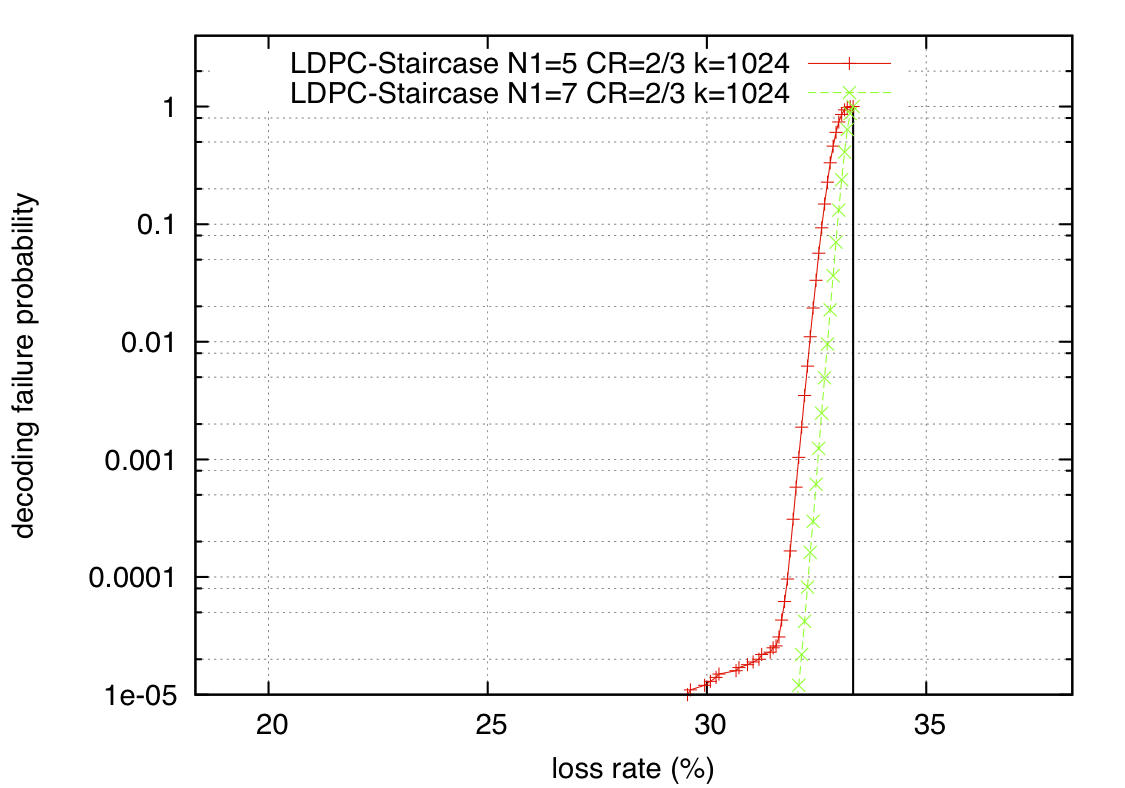
\includegraphics[width=0.45\linewidth]{dec_error_proba_wrt_loss_rate_n1_5_and_7_k_1024_cr_2_3.png}}
	\label{fig:fail_proba_wrt_loss_rate}
        }
        \subfigure[As a function of the number of received symbols]
        {
        {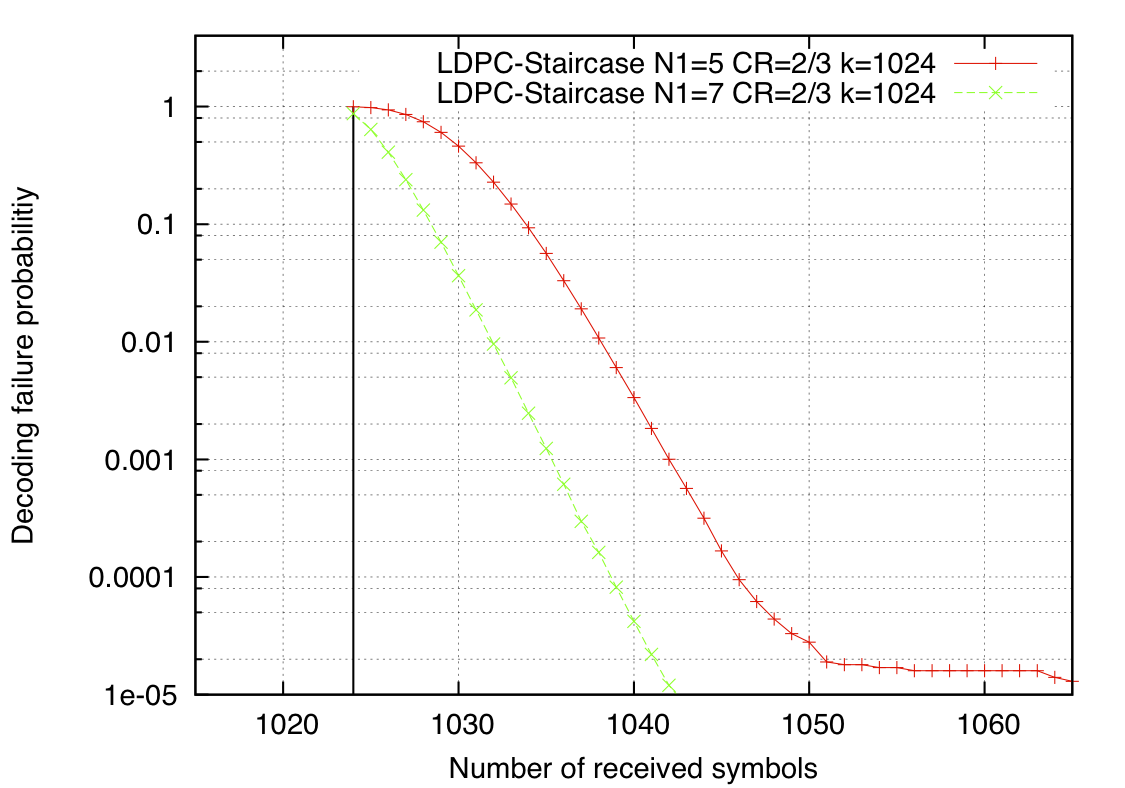
\includegraphics[width=0.45\linewidth]{dec_error_proba_wrt_overhead_n1_5_and_7_k_1024_cr_2_3.png}}
	\label{fig:fail_proba_wrt_nb_rx}
        }
	\caption{Example of decoding failure probability curve (LDPC-Staircase, $k=1.024$ symbols,
		code rate $2/3$, $N1=5$ or $7$).}
        \label{fig:failure_proba}
\end{figure}

% \begin{figure}[ht]{
% 	\begin{centering}
% 	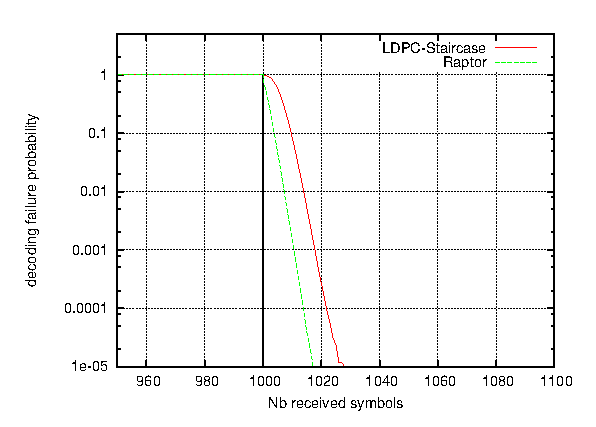
\includegraphics[scale=0.6]{failure_prob_wrt_nb_received.eps}\par
% 	\end{centering}
% 	\caption{Example of failure probability as a function of the number of received symbols.}
% 	\label{fig:failure_prob_wrt_nb_received}
% 	}
% \end{figure}

\subsection{Inefficiency ratio as a function of the code rate}
%-------------------------------------------------------------

In this curve, the object size is fixed.

Note that if in theory the \verb+inefficiency ratio+ of MDS codes is equal to $1$, this is
no longer true if there are several blocks and with certain transmission types.
For instance, using Reed-Solomon over an object that is composed of 5000 source symbols
(which leads to the creation of 30 blocks of size 166 or 167 source symbols each), and
using a random permutation of all symbols before transmitting, the resulting inefficiency
ratio is around $8\%$:
\verb+eperftool -codec=1 -tot_src=5000 -tot_rep=2500 -tx_type=0+
In that case, LDPC-staircase codes largely outperform Reed-Solomon codes\ldots


\subsection{Inefficiency ratio as a function of the object size}
%---------------------------------------------------------------

In this curve, the code rate is fixed.


\subsection{Number of XOR operations as a function of the object size}
%---------------------------------------------------------------------

{\bf (Valid only in Debug mode)}

This curve represents the number of operations (e.g. \verb+XOR+ on symbols) required to decode as
a function of the object size.
You have to use the \verb+Debug+ mode for the openfec library, because in \verb+Release+ mode,
statistics on operations are not enabled.
This curve gives a complementary view of the code and codec decoding speed, by focusing on
its internal complexity rather than speed.


\subsection{Number of XOR operations as a function of the channel loss percentage}
%---------------------------------------------------------------------------------

{\bf (Valid only in Debug mode)}

This is the same kind of curve as the previous one, but the object size is fixed.


%\newpage

%-------------------------------------------------------------------------------

\section{Plotting LDPC matrices}
%-------------------------------
\label{sec:plot_matrices}

\begin{flushright}
\framebox{
\begin{minipage}{10cm}
	\emph{$\rightarrow$ In short:
	OpenFEC includes the possibility to plot LDPC parity check matrices.
	}
\end{minipage}
}
\end{flushright}

An LDPC parity check matrix can be plot for analysis purposes.
To do so:

\begin{itemize}
\item If you are interested by plotting LDPC-staircase parity check matrix,
	then edit file:\\
	\verb+src/lib_stable/ldpc_staircase/of_codec_profile.h+.\\
	Define: \verb+#define IL_SUPPORT+\\
	Do the same for all LDPC codecs you are interested in (codecs are independent).

\item Edit file \verb+src/lib_stable/CMakeLists.txt+.\\
	Un-comment line: \verb+#target_link_libraries(openfec pthread IL)+ \\
	(and of course comment the similar line that omits IL) to make sure the
	(Dev)IL library be used during link edition.
\item Make sure DevIL library is installed on your machine. On a Linux machine,
	you can look for \verb+libIL.so+ to check it (e.g. use command
	\verb+locate libIL+ and look at the output).
	If not, you can either use a package management system (\verb+yum+ or similar),
	or install everything manually. To that purpose go to URL: \\
	\href{http://openil.sourceforge.net}{http://openil.sourceforge.net}\\
	and install the library as indicated.
\item Compile the library and tools in \verb+DEBUG+ mode, using: \\
\verb+cd build+ \\
\verb+cmake .. -DDEBUG:STRING=ON+\\
\verb+make+ \\
\item Launch eperftool, using one of the LDPC codes. A \verb+.bmp+ file is
	created in the local directory, containing an image of the parity
	check matrix. Open it with an appropriate tool (e.g. \verb+okular+ or \verb+eog+
	on a Linux machine).
	You can also launch automatically the visualisation tool, from OpenFEC,
	using the \verb+system("eog IL_file_image.bmp");+ call (for instance).
\end{itemize}

\begin{figure}[ht]{
	\begin{centering}
	
\includegraphics[scale=0.4]{IL_file_image-inverted.eps}\par
	\end{centering}
	\caption{Example of matrix (LDPC-staircase H matrix, with k=500, n=750)
	shown in reverse order ($H_2$, the double diagonal sub-matrix, appears before $H_1$).}
	\label{fig:plot_matrices_exple}
	}
\end{figure}

NB~1: For internal reasons, LDPC parity check matrices, $H = {H_1 | H_2}$ are often
stored in reverse order and $H_2$ (double diagonal sub-matrix in case of LDPC-Staircase)
appears before $H_1$.

NB~2: You can of course use image manipulation tools (e.g. \verb+gimp+) if you prefer
a negative view of the matrix (by default "1"s appear as white pixels, over a black
background, the example of figure~\ref{fig:plot_matrices_exple} is for instance inverted).


%\bibliographystyle{abbrv}
%\bibliography{biblio}

\end{document}
